\documentclass{article}

\usepackage{graphicx}
\usepackage{tikz}
\usepackage{tikzsymbols}
\usetikzlibrary{calc,patterns,shapes.geometric}
\pagestyle{empty}
\usepackage[margin=0pt]{geometry}
\geometry{papersize={14in,12in}}

\def\centerarc[#1](#2)(#3:#4:#5){\draw[#1] ($(#2)+({#5*cos(#3)},{#5*sin(#3)})$) arc (#3:#4:#5);}

\begin{document}
	\begin{figure}
		\centering
		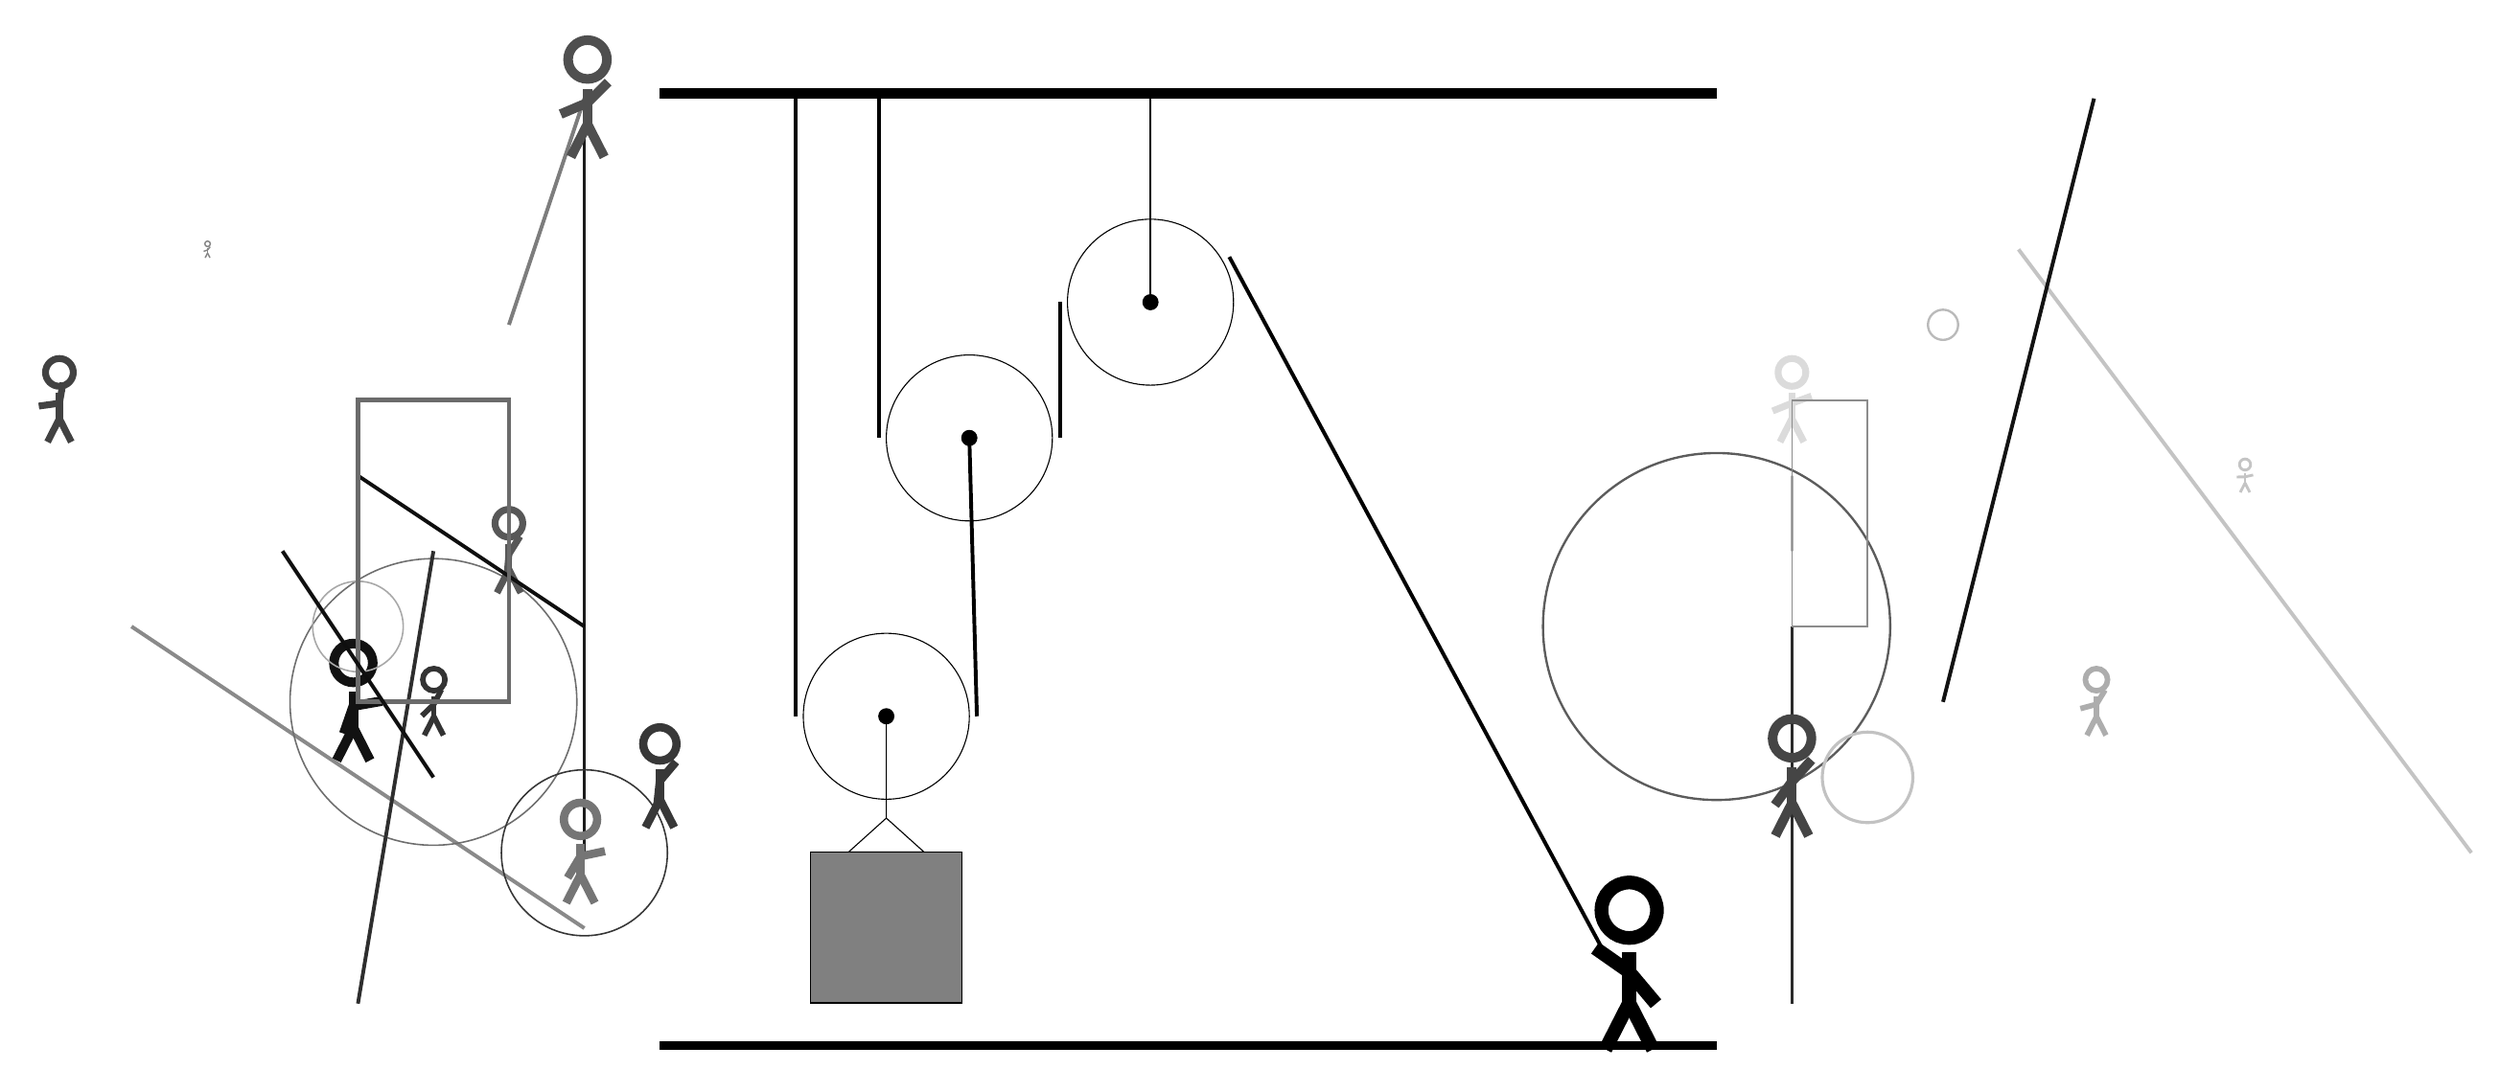
\begin{tikzpicture}
			%%%%% START %%%%%
			
			\draw[fill=black] (-2, 9) rectangle (12, 9.125);
			
			\draw (1, 0.81) circle (1.1);
			\draw[fill=black] (1, 0.81) circle (0.1);
			
			\node[line width=0.7mm, color=black!48] at (-8, 7) {\Strichmaxerl[1][20][51]};
			
			\draw[line width=0.5mm, color=black!46](-3, -2) -- (-9, 2);
			\node[line width=0.2mm, color=black!32] at (17, 1) {\Strichmaxerl[4][15][59]};
			\node[line width=0.7mm, color=black!80] at (-5, 1) {\Strichmaxerl[4][44][63]};
			\draw [line width=0.3mm, color=black!27](15, 6) circle (0.2);
			\draw[line width=0.3mm, color=black!32] (13, 3) rectangle (13, 4);
			\draw [line width=0.3mm, color=black!64](12, 2) circle (2.3);
			
			\node[line width=0.3mm, color=black!23] at (19, 4) {\Strichmaxerl[2][1][13]};
			\draw[line width=0.3mm, color=black!83] (13, 2) rectangle (13, -3);
			
			\node[line width=0.4mm, color=black!14] at (13, 5) {\Strichmaxerl[5][22][20]};
			
			\node[line width=0.6mm, color=black!93] at (-6, 1) {\Strichmaxerl[7][71][10]};
			\draw [line width=0.2mm, color=black!57](-5, 1) circle (1.9);
			\draw[line width=0.5mm, color=black!82](-6, -3) -- (-5, 3);
			
			\draw[line width=0.5mm, color=black!23](16, 7) -- (22, -1);
			\draw[line width=0.2mm, color=black!45] (13, 5) rectangle (14, 2);
			\node[line width=0.2mm, color=black!66] at (-4, 3) {\Strichmaxerl[5][85][58]};
			
			\draw[line width=0.5mm, color=black!51](-3, 9) -- (-4, 6);
			\draw [line width=0.2mm, color=black!34](-6, 2) circle (0.6);
			\draw[line width=0.4mm, color=black!89] (-3, 9) rectangle (-3, -1);
			
			\node[line width=0.2mm, color=black!78] at (-2, 0) {\Strichmaxerl[6][84][50]};
			\draw[line width=0.5mm, color=black!94](-6, 4) -- (-3, 2);
			
			\draw[line width=0.5mm, color=black!93](15, 1) -- (17, 9);
			\draw [line width=0.2mm, color=black!79](-3, -1) circle (1.1);
			\draw [line width=0.4mm, color=black!24](14, 0) circle (0.6);
			\node[line width=0.5mm, color=black!54] at (-3, -1) {\Strichmaxerl[6][59][12]};
			\draw[line width=0.6mm, color=black!58] (-4, 5) rectangle (-6, 1);
			\node[line width=0.4mm, color=black!74] at (-10, 5) {\Strichmaxerl[5][8][80]};
			\node[line width=0.2mm, color=black!69] at (-3, 9) {\Strichmaxerl[7][23][45]};
			\draw[line width=0.5mm, color=black!94](-5, 0) -- (-7, 3);
			
			\node[line width=0.6mm, color=black!73] at (13, 0) {\Strichmaxerl[7][54][48]};
			
			\draw (2.1, 4.5) circle (1.1);
			\draw[fill=black] (2.1, 4.5) circle (0.1);
			
			\draw (4.5, 6.3) circle (1.1);
			\draw[fill=black] (4.5, 6.3) circle (0.1);
			\draw[thick] (4.5, 6.3) -- (4.5, 9);
			
			\draw (1, 0.81) -- (1, -0.54) -- (0.5, -0.99) -- (1.5, -0.99) -- (1, -0.54);
			\draw[fill=black!50] (0, -0.99) rectangle (2, -2.99);
			
			\draw[line width=0.5mm] (-0.2, 9) -- (-0.2, 0.81);
			\centerarc[line width=0.5mm](1, 0.81)(180:360:1.2000000000000002);
			\draw[line width=0.5mm](2.2, 0.81) -- (2.1, 4.5);
			\draw[line width=0.5mm] (0.9, 9) -- (0.9, 4.5);
			\centerarc[line width=0.5mm](2.1, 4.5)(180:360:1.2000000000000002);
			\draw[line width=0.5mm](3.3, 4.5) -- (3.3, 6.3);
			\centerarc[line width=0.5mm](4.5, 6.3)(30:180:1.2000000000000002);
			\draw[line width=0.5mm] (5.544, 6.9) -- (10.5, -2.3);
			
			\node at (10.8, -2.5) {\Strichmaxerl[10][-35][-50]};
			
			\draw[fill=black] (-2, -3.5) rectangle (12, -3.6);
			
			%%%%% END %%%%%
		\end{tikzpicture}
	\end{figure}	
\end{document}